% !TEX program = xelatex
\documentclass[a4paper,14pt,oneside,openany]{memoir}

%%% Задаем поля, отступы и межстрочный интервал %%%

\usepackage[left=30mm, right=15mm, top=20mm, bottom=20mm]{geometry}
\pagestyle{plain}
\parindent=1.25cm
\usepackage{indentfirst}

%%% Задаем языковые параметры и шрифт %%%

\usepackage[english,russian]{babel}
\babelfont[russian]{rm}{Times New Roman}
\babelfont[russian]{tt}{Courier New}

%%% Задаем стиль заголовков и подзаголовков в тексте %%%

\setsecnumdepth{subsection}
\renewcommand*{\chapterheadstart}{}
\renewcommand*{\printchaptername}{}
\renewcommand*{\chapnumfont}{\normalfont\bfseries}
\renewcommand*{\afterchapternum}{\hspace{1em}}
\renewcommand*{\printchaptertitle}{\normalfont\bfseries\centering\MakeUppercase}
\setbeforesecskip{20pt}
\setaftersecskip{20pt}
\setsecheadstyle{\raggedright\normalfont\bfseries}
\setbeforesubsecskip{20pt}
\setaftersubsecskip{20pt}
\setsubsecheadstyle{\raggedright\normalfont\bfseries}

%%% Исправление нумерации секций %%%

\renewcommand{\thesection}{\arabic{section}}
\renewcommand{\thesubsection}{\arabic{subsection}}

%%% Сквозная нумерация рисунков и таблиц %%%

\counterwithout{figure}{chapter}
\counterwithout{table}{chapter}

%%% Выравнивание и переносы %%%

\tolerance 1414
\hbadness 1414
\emergencystretch 1.5em
\clubpenalty=10000
\widowpenalty=10000

%%% Задаем параметры оформления рисунков и таблиц %%%

\usepackage{graphicx}
\usepackage{caption}
\usepackage{subcaption}
\usepackage{float}
\graphicspath{{photo/}}
\captionsetup[figure]{font=small, width=\textwidth, name=Рисунок, justification=centering}
\captiondelim{ --- }
\usepackage[section]{placeins}

%%% Задаем параметры ссылок и гиперссылок %%% 

\usepackage{hyperref}
\hypersetup{
    colorlinks=true,
    linkcolor=red,
    citecolor=red
}

%%% Настраиваем отображение списков %%%

\usepackage{enumitem}
\renewcommand*{\labelitemi}{\normalfont{--}}
\setlist{noitemsep, leftmargin=*}

\begin{document}

% Титульный лист (без номера страницы)
\thispagestyle{empty}

\begin{center}
    МИНИСТЕРСТВО ЦИФРОВОГО РАЗВИТИЯ, СВЯЗИ И МАССОВЫХ \\ КОММУНИКАЦИЙ \\ РОССИЙСКОЙ ФЕДЕРАЦИИ

    \vspace{20pt}

    Федеральное государственное бюджетное образовательное учреждение \\ высшего образования \\
    "Сибирский государственный университет телекоммуникаций и \\ информатики"

    \vspace{20pt}

    Кафедра телекоммуникационных систем и вычислительных средств \\ (ТС и ВС)
\end{center}

\vfill

\begin{center}
    Практическая работа №4 \\
    по дисциплине \\
    \textit{"Web-технологии"}

    \vspace{20pt}

    по теме: \\
    \uppercase{Настройка шлюза локальной сети на базе Ubuntu}
\end{center}

\vfill

\noindent Студент: \\
\textit{Группа ИКС-532 \hfill А.С. Лёшин}

\vspace{20pt}

\noindent Преподаватель: \\
\textit{старший преподаватель \hfill А.В. Андреев}

\vfill

\begin{center}
    Новосибирск 2026 г.
\end{center}

\newpage
\setcounter{page}{2}
\OnehalfSpacing*

\section*{Введение}
\addcontentsline{toc}{section}{Введение}

Целью работы является создание функционального шлюза, обеспечивающего:
\begin{itemize}
    \item маршрутизацию трафика между локальной сетью и интернетом;
    \item автоматическую выдачу сетевых настроек клиентам;
    \item доступ в интернет для всех устройств локальной сети.
\end{itemize}

\section{Настройка сетевого шлюза на базе Ubuntu}

\subsection{Конфигурация сетевых интерфейсов}

Первым этапом настройки шлюза является конфигурирование сетевых интерфейсов сервера. Для просмотра доступных интерфейсов используется команда \texttt{ip a}. На \hyperref[fig:interfaces]{рисунке \ref*{fig:interfaces}} представлен список сетевых интерфейсов, где:
\begin{itemize}
    \item \texttt{enp0s8} — внешний интерфейс для связи с интернетом;
    \item \texttt{enp0s9} — внутренний интерфейс для построения локальной сети.
\end{itemize}

\begin{figure}[H]
    \centering
    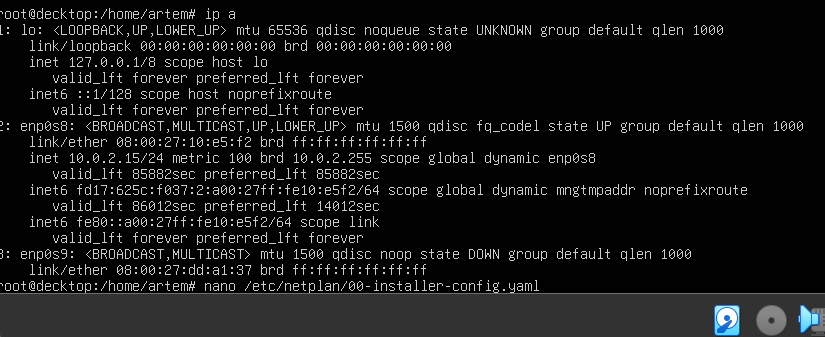
\includegraphics[width=0.8\textwidth]{photo/screen1.png}
    \caption{Список сетевых интерфейсов}
    \label{fig:interfaces}
\end{figure}

После определения интерфейсов необходимо отредактировать их настройки. На \hyperref[fig:config]{рисунке \ref*{fig:config}} показаны параметры, заданные для интерфейсов \texttt{enp0s8} и \texttt{enp0s9}.

\begin{figure}[H]
    \centering
    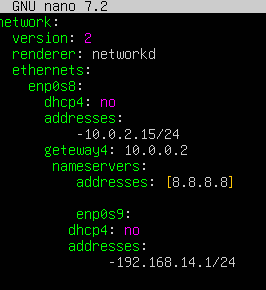
\includegraphics[width=0.6\textwidth]{photo/screen2.png}
    \caption{Настройка сетевых интерфейсов enp0s8 и enp0s9}
    \label{fig:config}
\end{figure}

\subsection{Проверка работоспособности сети}

Для проверки правильности настройки интерфейсов используется команда \texttt{ip a}, результат выполнения которой представлен на \hyperref[fig:ip]{рисунке \ref*{fig:ip}}.

\begin{figure}[H]
    \centering
    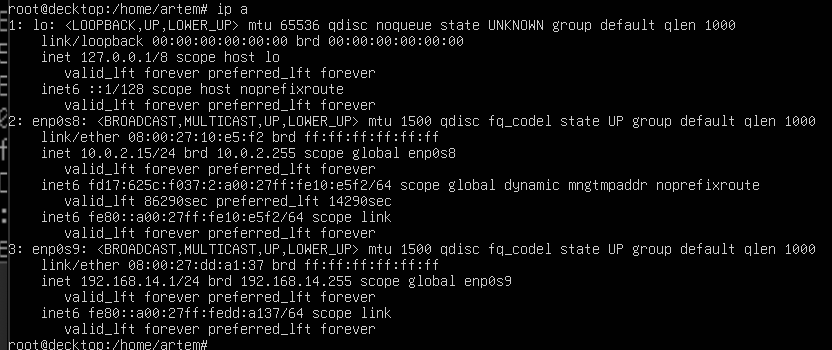
\includegraphics[width=0.8\textwidth]{photo/screen3.png}
    \caption{Результат выполнения команды ip a}
    \label{fig:ip}
\end{figure}

Наличие связи с внешними ресурсами проверяется командой \texttt{ping}. На \hyperref[fig:ping]{рисунке \ref*{fig:ping}} продемонстрирован успешный обмен пакетами с ресурсом \texttt{ya.ru}.

\begin{figure}[H]
    \centering
    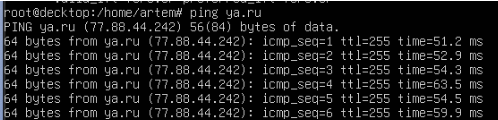
\includegraphics[width=0.8\textwidth]{photo/screen4.png}
    \caption{Проверка связи с ya.ru}
    \label{fig:ping}
\end{figure}

\subsection{Настройка тестового клиента}

Для корректной работы в локальной сети клиенту присваиваются следующие параметры:
\begin{itemize}
    \item IP-адрес: 192.168.14.10;
    \item маска подсети: 255.255.255.0;
    \item шлюз по умолчанию: 192.168.14.1;
    \item DNS-сервер: 192.168.14.1.
\end{itemize}

На \hyperref[fig:client]{рисунке \ref*{fig:client}} представлен интерфейс настройки сети клиентской системы.

\begin{figure}[H]
    \centering
    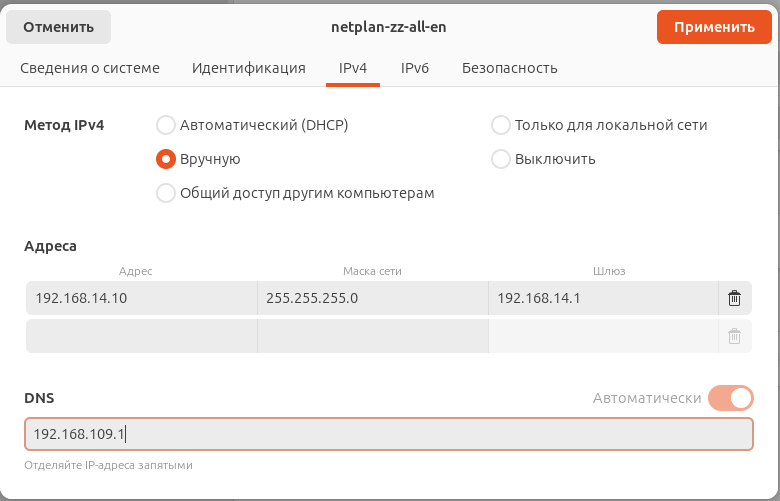
\includegraphics[width=0.7\textwidth]{photo/screen5.png}
    \caption{Настройка сети на клиентском устройстве}
    \label{fig:client}
\end{figure}

\subsection{Включение маршрутизации и настройка фаервола}

Для проверки связи между клиентом и шлюзом выполняется команда \texttt{ping 192.168.14.1}. На \hyperref[fig:ping-client]{рисунке \ref*{fig:ping-client}} видно, что запросы успешно выполняются.

\begin{figure}[H]
    \centering
    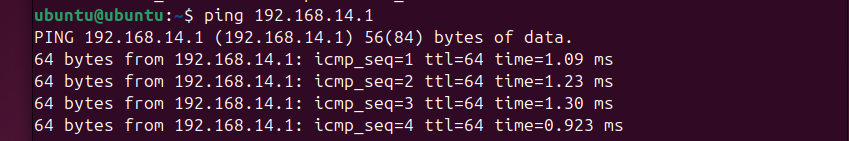
\includegraphics[width=0.8\textwidth]{photo/screen6.png}
    \caption{Проверка связи клиента со шлюзом}
    \label{fig:ping-client}
\end{figure}

Далее необходимо разрешить перенаправление пакетов на сервере-шлюзе. Для этого в файле \texttt{/etc/sysctl.conf} раскомментируется строка:

\begin{verbatim}
net.ipv4.ip_forward=1
\end{verbatim}

Для сохранения правил фаервола после перезагрузки используется пакет \texttt{iptables-persistent}. На \hyperref[fig:rules]{рисунке \ref*{fig:rules}} показан процесс создания правил.

\begin{figure}[H]
    \centering
    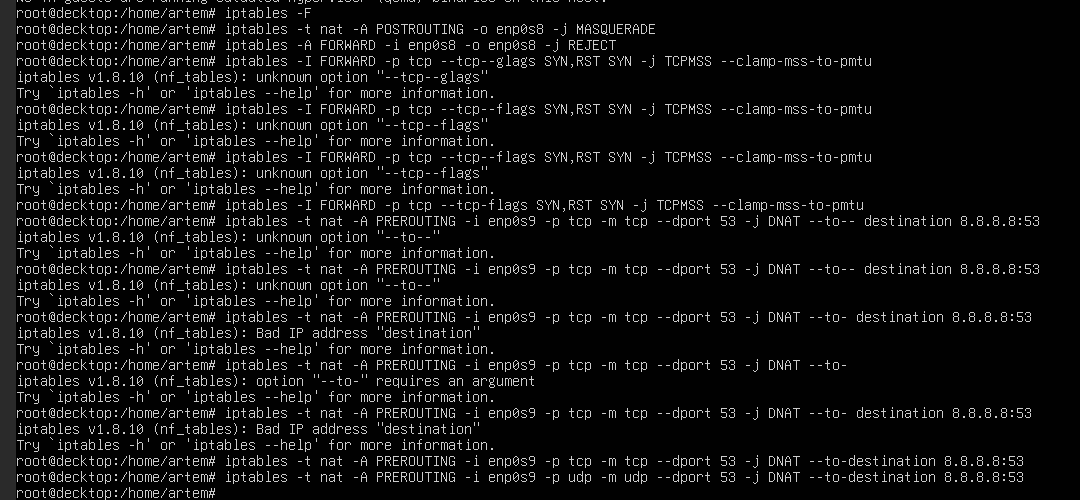
\includegraphics[width=0.6\textwidth]{photo/screen7.png}
    \caption{Создание правил iptables}
    \label{fig:rules}
\end{figure}

После перезагрузки сервера необходимо проверить доступность интернета с клиентского устройства. На \hyperref[fig:ethernet]{рисунке \ref*{fig:ethernet}} представлен результат открытия веб-страницы на клиентской системе, что подтверждает корректную работу шлюза.

\begin{figure}[H]
    \centering
    
\includegraphics[width=0.7\textwidth]{photo/screen8.png}
    \caption{Доступ в интернет с клиентского устройства}
    \label{fig:ethernet}
\end{figure}

\section{Настройка DHCP-сервера}

\subsection{Установка DHCP-сервера}

Для автоматической раздачи сетевых настроек устройствам локальной сети настраивается DHCP-сервер. Процесс установки выполняется следующими командами:
\begin{verbatim}
sudo su
apt-get update
apt install isc-dhcp-server
\end{verbatim}

Пакет \texttt{isc-dhcp-server} устанавливается вместе со всеми необходимыми зависимостями. Адресное пространство локальной сети определено в диапазоне \texttt{192.168.14.0/24}, что позволяет подключать до 254 сетевых устройств.

\subsection{Конфигурирование DHCP-сервера}

На первом этапе необходимо указать интерфейс, на котором будет работать DHCP-сервер. В файле \texttt{/etc/default/isc-dhcp-server} задается параметр:
\begin{verbatim}
INTERFACESv4="enp0s9"
\end{verbatim}

Далее выполняется настройка конфигурационного файла. На \hyperref[fig:subnet]{рисунке \ref*{fig:subnet}} представлен фрагмент конфигурационного файла с описанием подсети.

\begin{figure}[H]
    \centering
    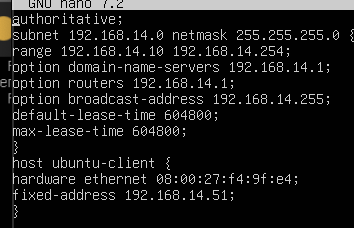
\includegraphics[width=0.8\textwidth]{photo/screen9.png}
    \caption{Конфигурация подсети в DHCP-сервере}
    \label{fig:subnet}
\end{figure}

\subsection{Запуск и проверка DHCP-сервера}

После сохранения конфигурации запускается сервис DHCP:
\begin{verbatim}
service isc-dhcp-server start
\end{verbatim}

Статус сервиса проверяется командой:
\begin{verbatim}
service isc-dhcp-server status
\end{verbatim}

На \hyperref[fig:status]{рисунке \ref*{fig:status}} отображен результат проверки, подтверждающий успешный запуск DHCP-сервера.

\begin{figure}[H]
    \centering
    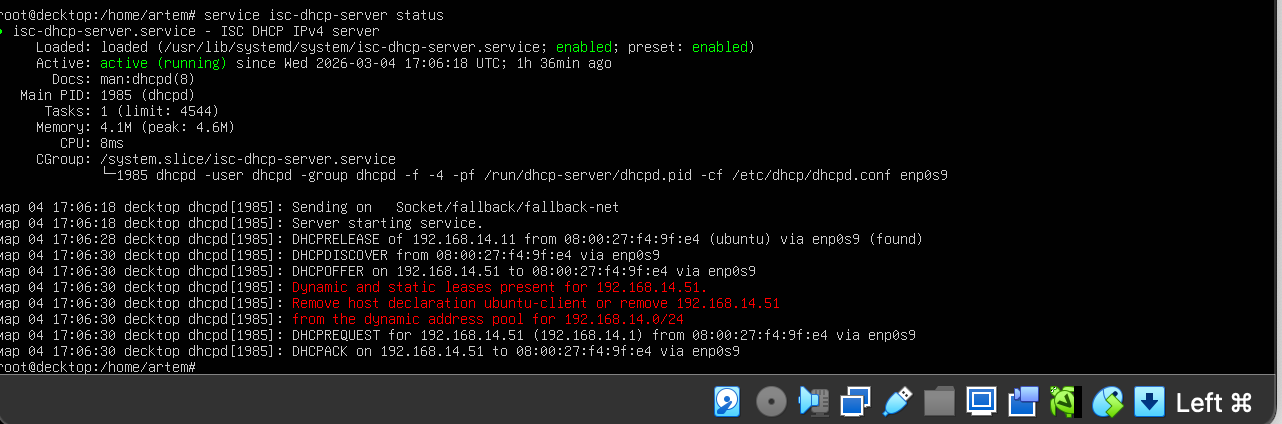
\includegraphics[width=0.8\textwidth]{photo/screen10.png}
    \caption{Статус работы DHCP-сервера}
    \label{fig:status}
\end{figure}

\subsection{Итоговая проверка}

В результате выполнения всех настроек должна быть обеспечена связь между сервером и клиентскими устройствами, а также доступ в интернет. На \hyperref[fig:examination]{рисунке \ref*{fig:examination}} представлены результаты проверки, подтверждающие корректную работу всех настроенных компонентов.

\begin{figure}[H]
    \centering
    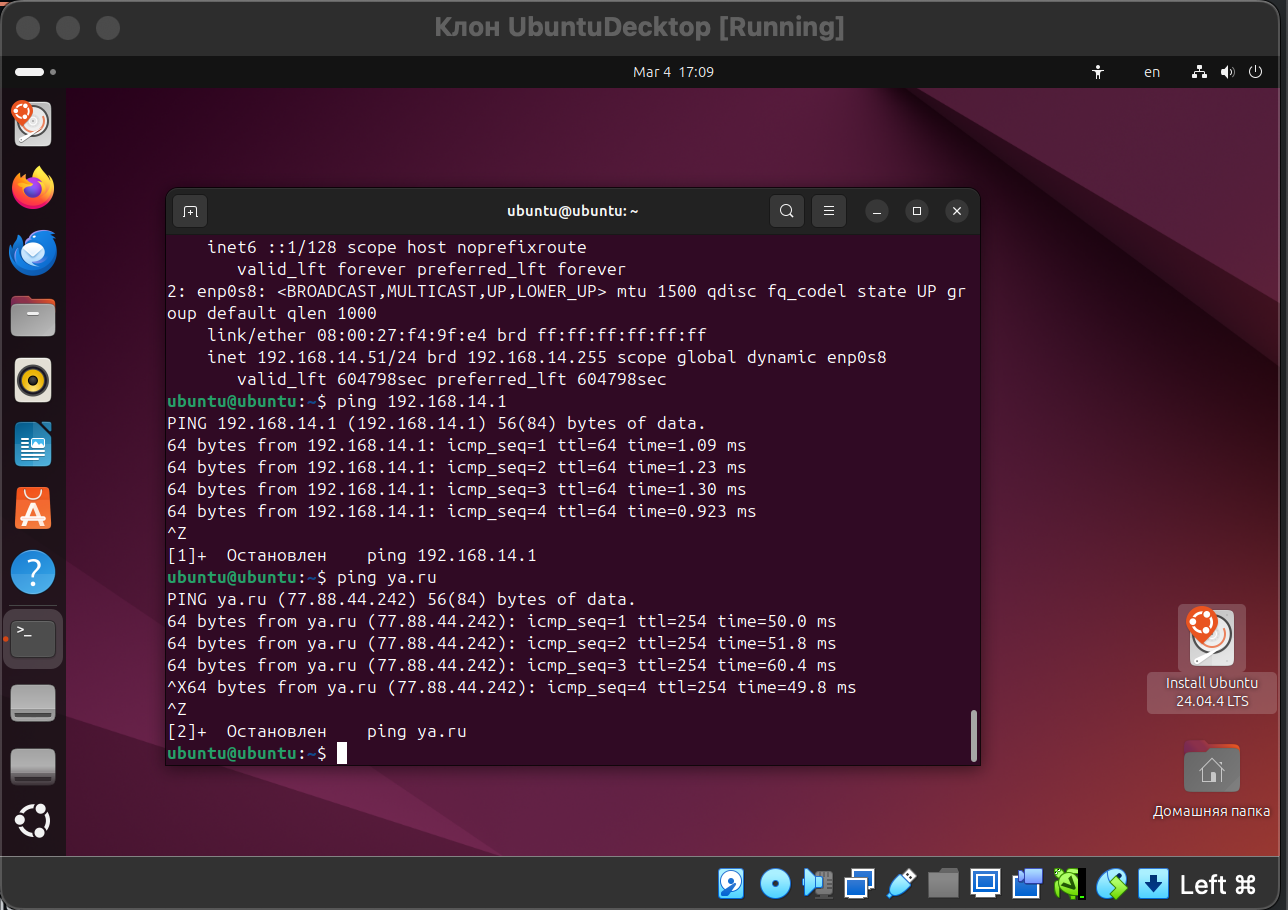
\includegraphics[width=0.8\textwidth]{photo/screen11.png}
    \caption{Результаты итоговой проверки}
    \label{fig:examination}
\end{figure}

\section*{Заключение}
\addcontentsline{toc}{section}{Заключение}

В ходе выполнения работы был настроен сетевой шлюз на базе операционной системы Ubuntu. Выполнены следующие задачи:
\begin{enumerate}
    \item сконфигурированы сетевые интерфейсы сервера с разделением на внешний и внутренний;
    \item настроена маршрутизация трафика между локальной сетью и интернетом;
    \item установлен и сконфигурирован DHCP-сервер для автоматической раздачи IP-адресов;
    \item выполнена проверка работоспособности всех компонентов.
\end{enumerate}

В результате проведённых настроек клиентские устройства локальной сети получают сетевые параметры автоматически и имеют полноценный доступ к интернету через настроенный шлюз.

\end{document}